%%%%%% DON'T MODIFY STARTING HERE
\newpage
\section*{2. Python API}

For this section, you may reference the template code or the \href{https://document.wlkata.com/?doc=/wlkata-mirobot-resources-for-education/python-sdk/}{documentation}. This \href{https://docs.google.com/document/d/1Jh17WoaQvjzbp1AMjOTzPfXSAxNnE87V8AEH1H-iLk8/edit?usp=sharing}{handbook} may also be useful for additional information.
For all subsequent exercises, we will create a Python virtual environment using \href{https://www.anaconda.com/products/individual}{Anaconda}.
Please install Anaconda as instructed in the above link, then create a new environment:
%
\begin{verbatim}
    conda create -n 52-O python=3.8
\end{verbatim}

Then activate this virtual environment. You must do this for all subsequent exercises even if not instructed.
\begin{verbatim}
    conda activate 52-O
\end{verbatim}

\paragraph{2A.} Install Python SDK: \texttt{pip install wlkata-mirobot-python}. Attach at screenshot that shows successful completion in the space provided.

\paragraph{2B.} Create robot arm object and home.
Attach a screenshot of successful command execution.
\begin{enumerate} %[(i)]
    \item \texttt{arm = WlkataMirobot(portname=``your port name")}
    \item \texttt{arm.home()}
\end{enumerate}

\paragraph{2C.} Replicate \textbf{1E} and \textbf{1F} using the Python API.
Consult the documentation to figure out the values for \texttt{joint\_angles}, \texttt{x, y, z}, etc.
Submit photo result and include your code in the space provided.
\begin{itemize}
    \item \texttt{def set\_joint\_angle(self, joint\_angles, is\_relative=False, speed=None, wait\_ok=None)}
    \item \texttt{def set\_tool\_pose(self, x=None, y=None, z=None, roll=0.0, pitch=0.0, yaw=0.0,  mode='p2p', speed=None, is\_relative=False, wait\_ok=True)}
\end{itemize}



\paragraph{2D} Utilize the below 4 interpolation functions to make the robot go from \texttt{TARGET A} to \texttt{TARGET B} on the mat.
Submit photo result of the arm in \textbf{both} targets in the space provided.
Please also include your code where appropriate.
% TODO
\begin{itemize}
    \item Point2Point: \texttt{def p2p\_interpolation(self, x=None, y=None, z=None, a=None, b=None, c=None, speed=None, is\_relative=False, wait\_ok=None)}
    \item Linear: \texttt{def linear\_interpolation(self, x=None, y=None, z=None, a=None, b=None, c=None, speed=None, is\_relative=False, wait\_ok=None)}
    \item Door: \texttt{def door\_interpolation(self, x=None, y=None, z=None, a=None, b=None, c=None, speed=None, is\_relative=False, wait\_ok=None)}
    \item Circular: \texttt{def circular\_interpolation(self, ex, ey, radius, is\_cw=True, speed=None, wait\_ok=None)}
\end{itemize}
%%%%%% DON'T MODIFY UNTIL HERE

\paragraph{Answers.}
Please do not exceed the height provided for each answer image.
%%%%%% YOU ANSWER STARTS HERE

% NOTE: MAKE SURE YOU DON'T CHANGE THE HEIGHT OF IMAGES
% NOTE: MAKE SURE TO REMOVE THE 'draft' OPTION FOR includegraphics BELOW. OTHERWISE, YOU WILL NOT SEE YOUR IMAGES.

\paragraph{2A. Install Python SDK}
\begin{center}
    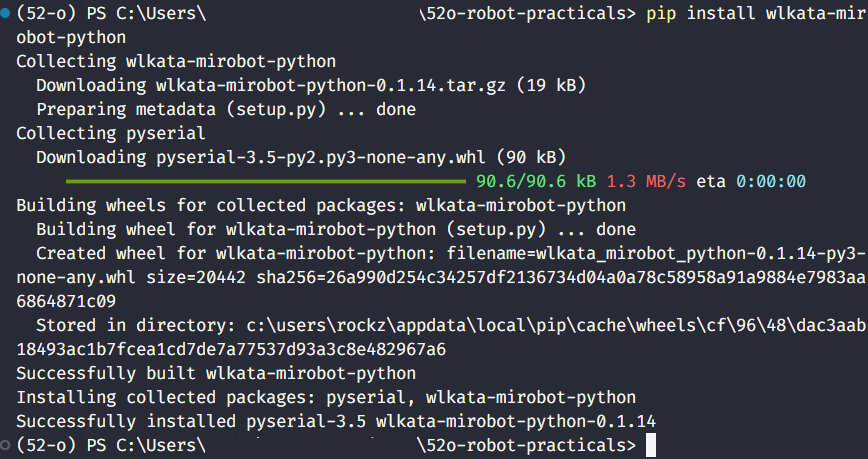
\includegraphics[height=2.5in]{image/2a_pythonsdk.png}
\end{center}

\paragraph{2B. Create Python Object and Home}
\begin{center}
    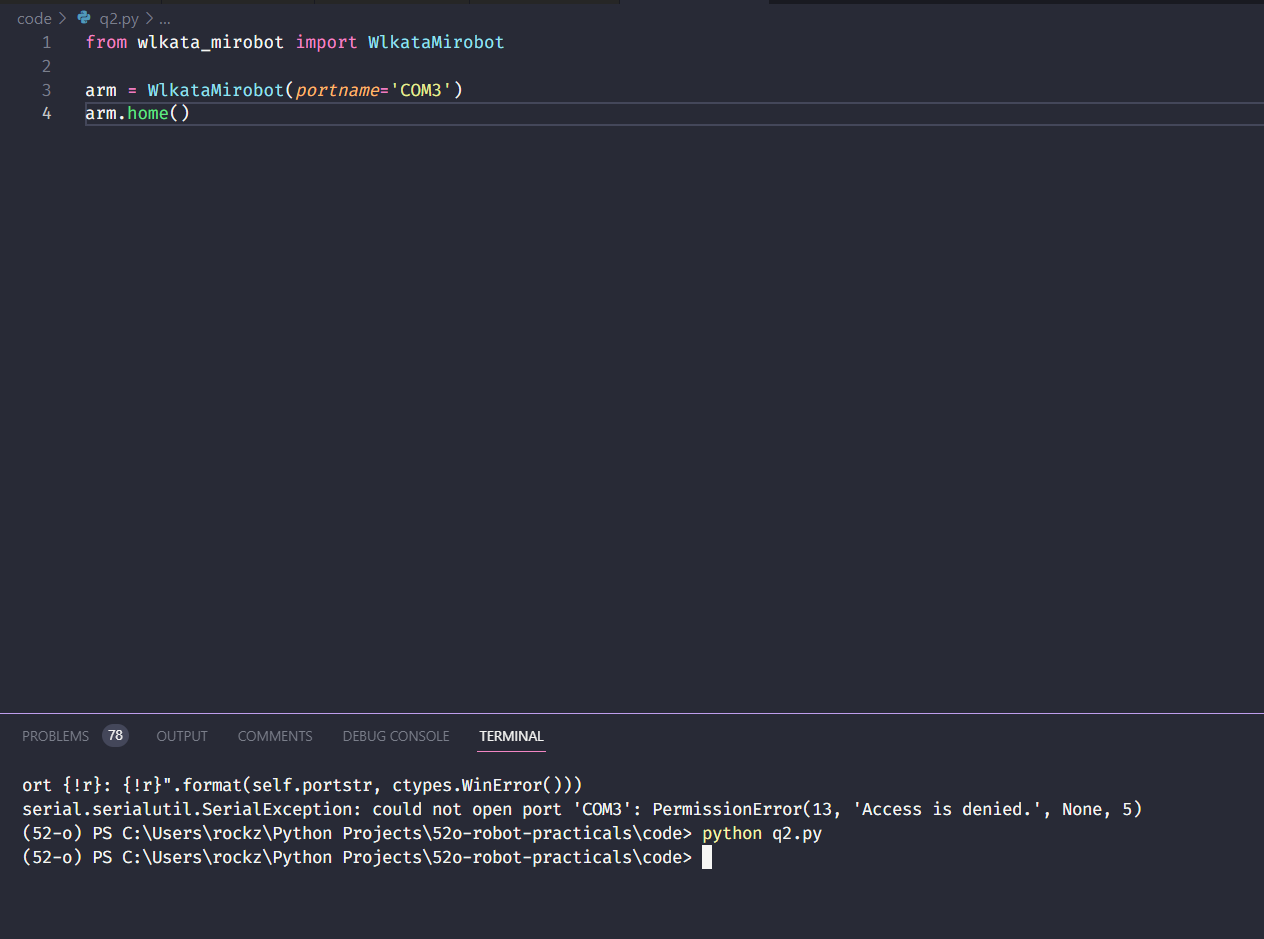
\includegraphics[height=2.5in]{image/2b_exec_success.png}
\end{center}

\newpage
\paragraph{2C. IK / FK using Python}
Include your code also.

\begin{figure}[hb!]
     \centering
    \begin{subfigure}[b]{0.3\textwidth}
        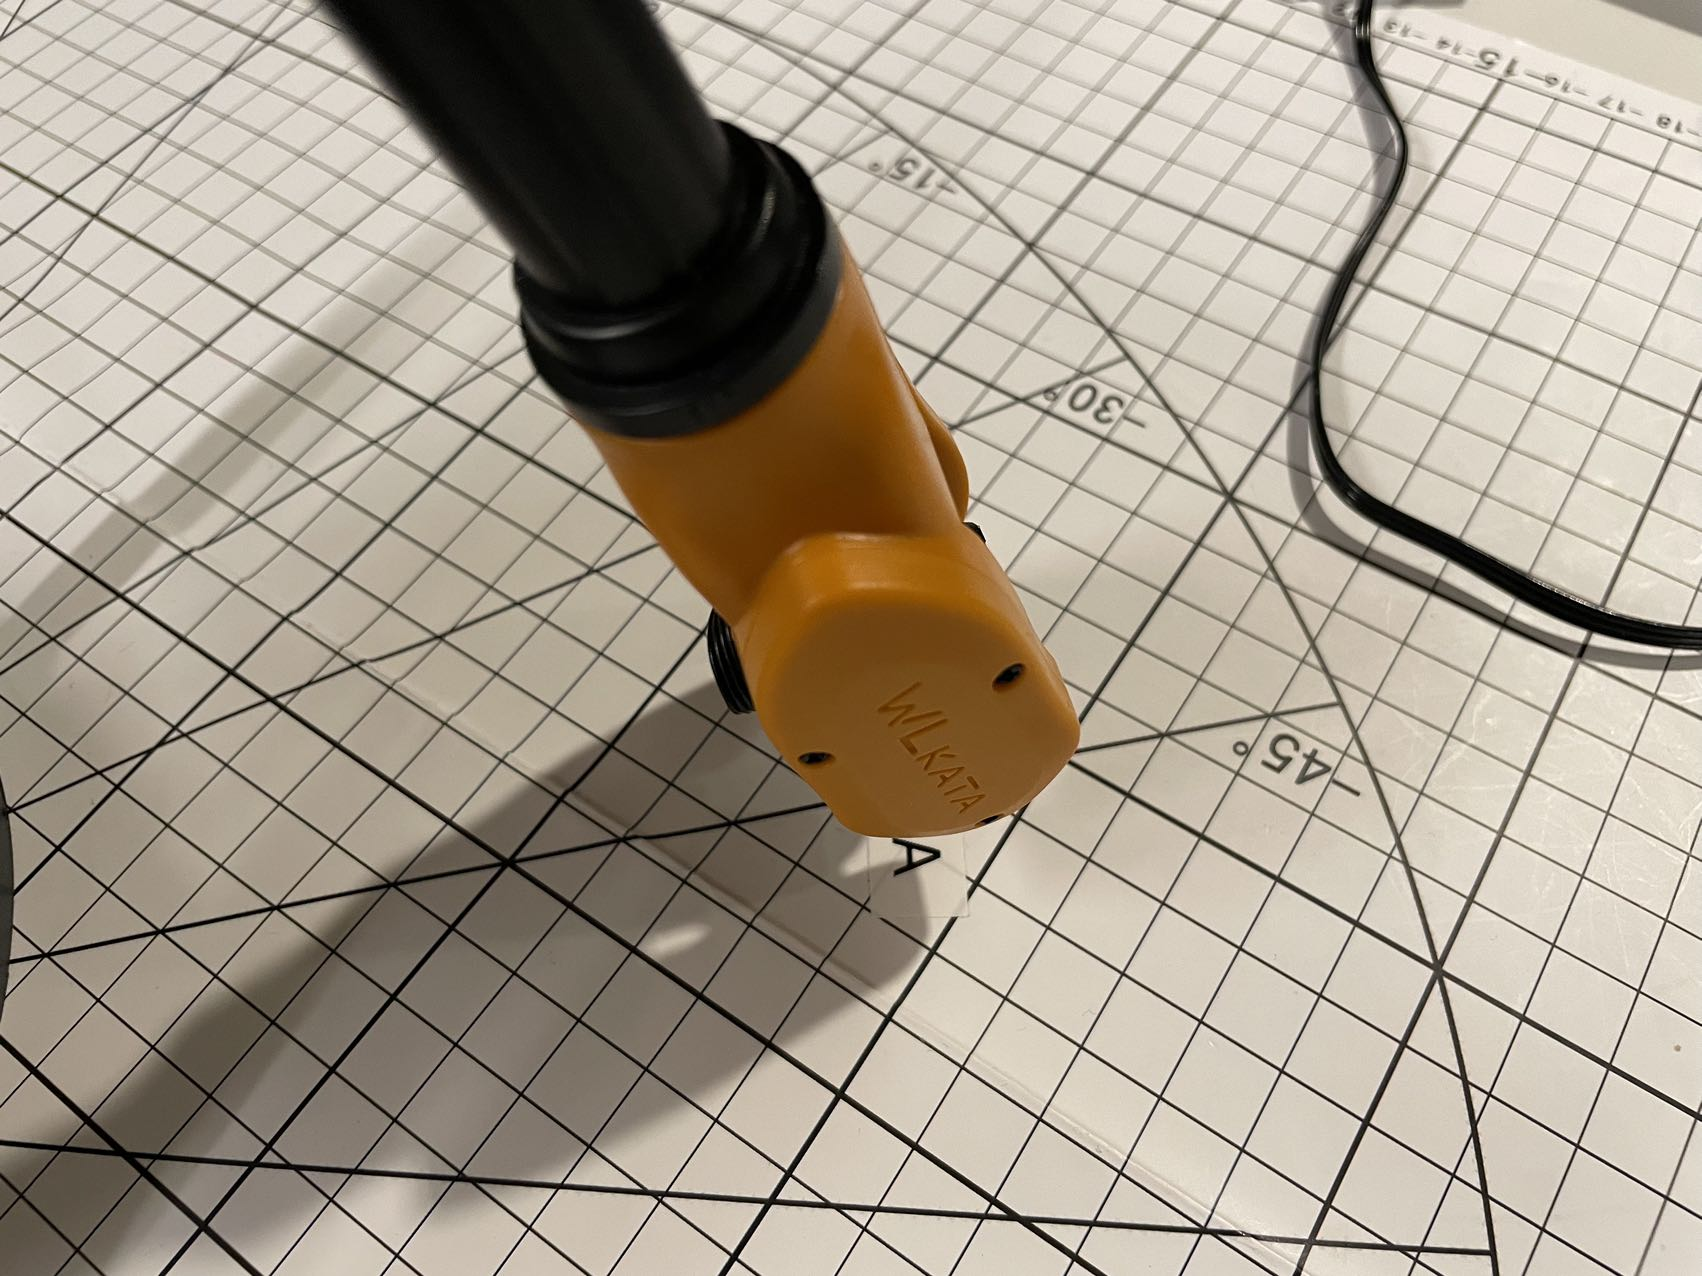
\includegraphics[height=2.5in]{image/2c_a.jpg}
         \caption*{Inverse Kinematics to \texttt{TARGET A}}
     \end{subfigure}
     %
     \hfill
     %
     \begin{subfigure}[b]{0.3\textwidth}
        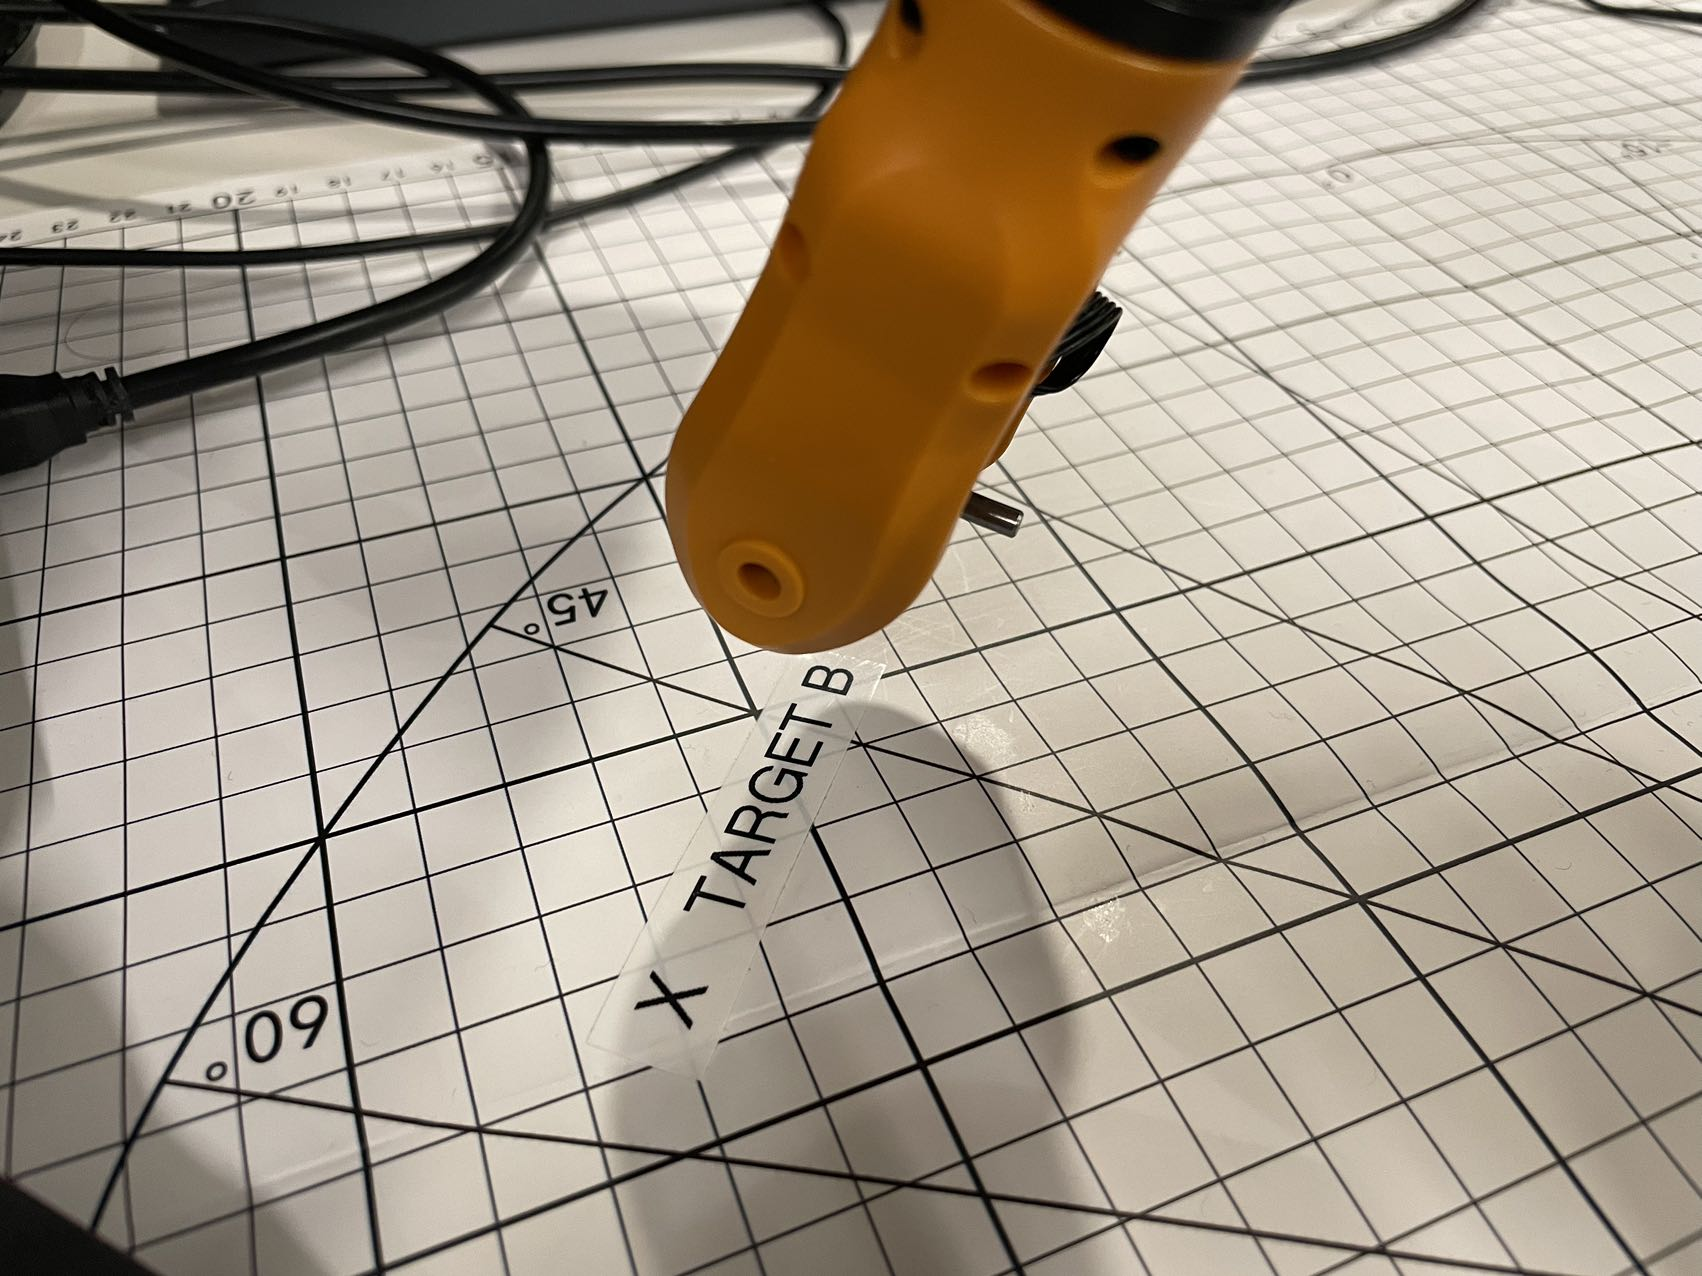
\includegraphics[height=2.5in]{image/2c_b.jpg}
         \caption*{Forward Kinematics to \texttt{TARGET B}}
     \end{subfigure}
    \caption*{Answer for 2C.}
\end{figure}

\begin{minted}{python}
from wlkata_mirobot import WlkataMirobot
import sys

arm = WlkataMirobot(portname='COM3')
arm.home()


if sys.argv[1] == '1e':
    arm.set_tool_pose(x=130,y=150,z=10)
if sys.argv[1] == '1f':
    angles = {1:135.0, 2:55.0, 3:10.0}
    arm.set_joint_angle(angles)
\end{minted}

\newpage
\paragraph{2D. Interpolation}
Include your code also.

\begin{figure}[hb!]
     \centering
    \begin{subfigure}[b]{0.3\textwidth}
        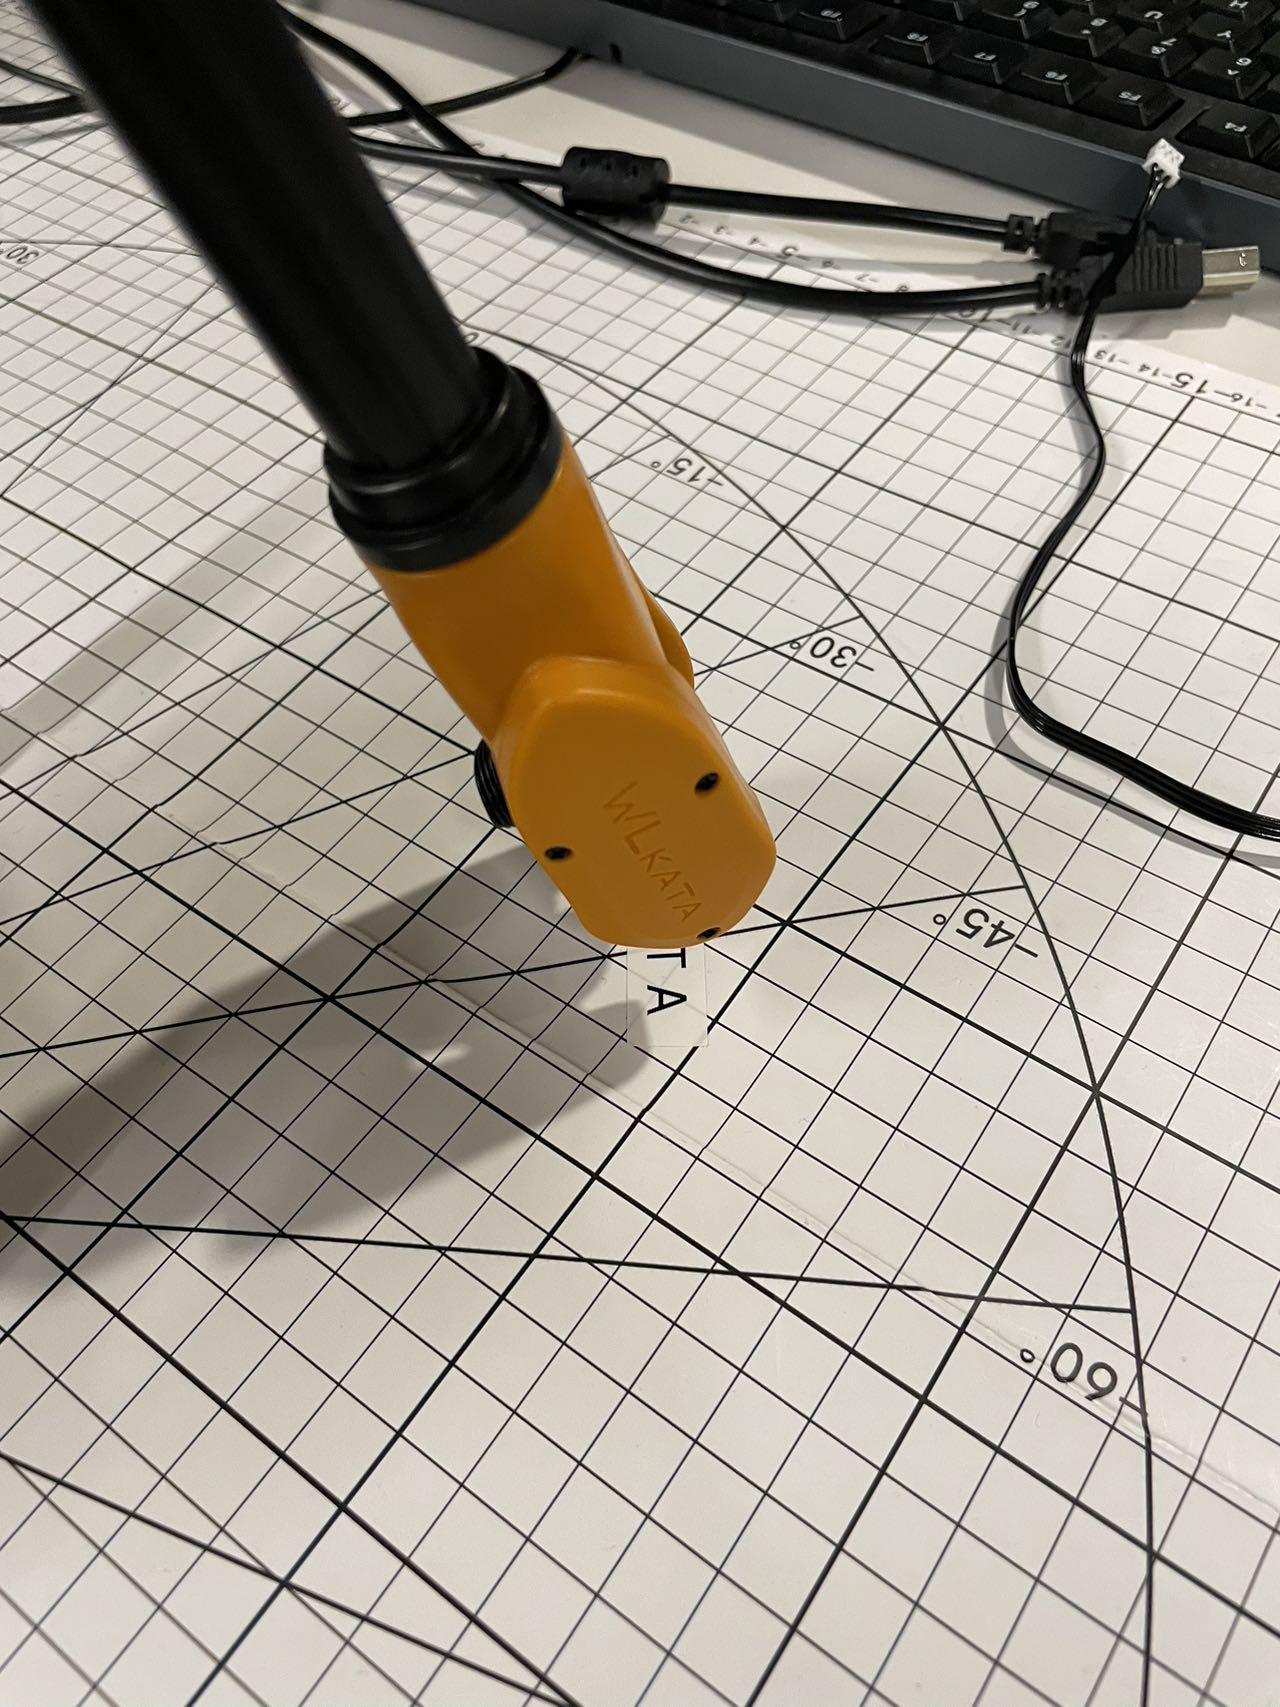
\includegraphics[height=2.5in]{image/2d_p2p.jpg}
         \caption*{Point2Point: \texttt{TARGET A}}
     \end{subfigure}
     %
     \hfill
     %
     \begin{subfigure}[b]{0.3\textwidth}
        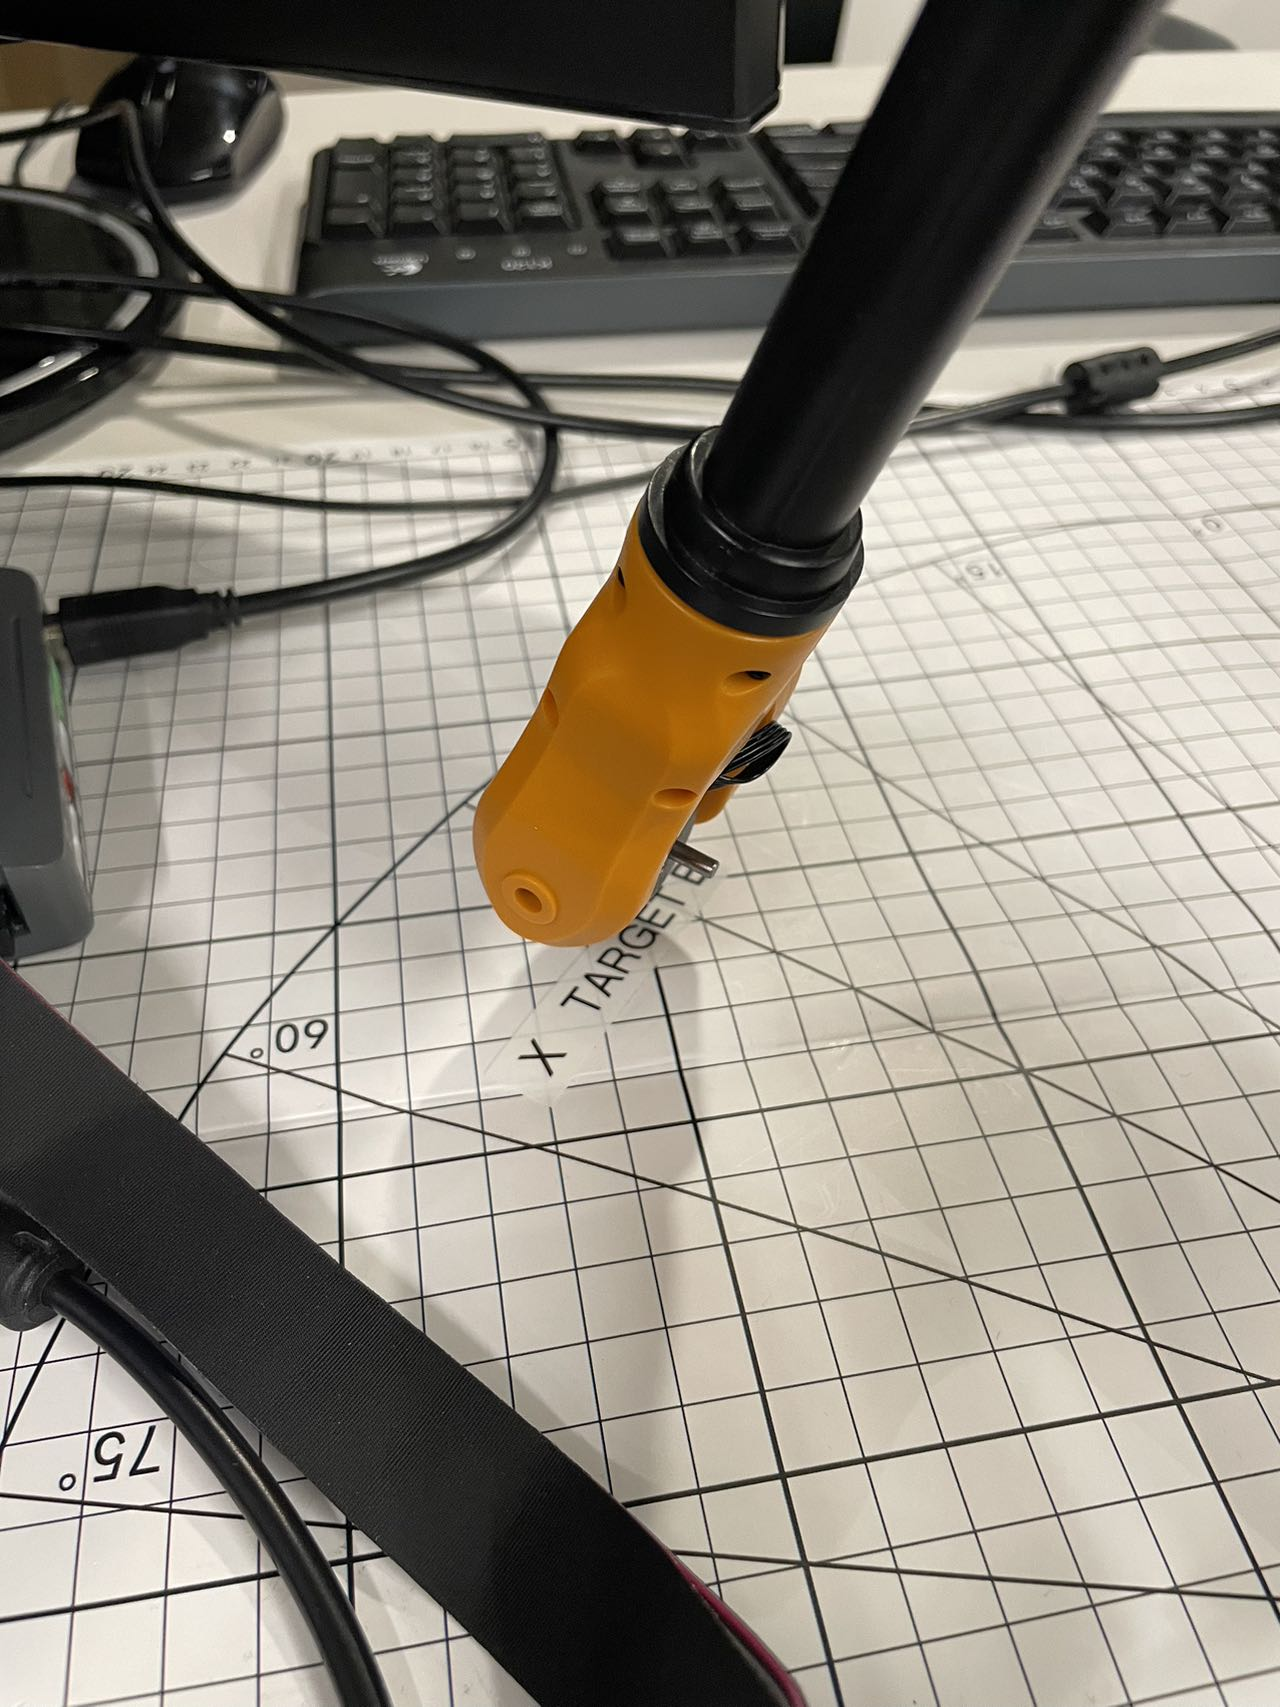
\includegraphics[height=2.5in]{image/2d_p2p_b.jpg}
         \caption*{Point2Point: \texttt{TARGET B}}
     \end{subfigure}
    \caption*{Answer for 2D.}
\end{figure}
%
\begin{minted}{python}
#Common header part skipped

if sys.argv[1] == 'p2p':
    # Go to A
    arm.p2p_interpolation(x=130.0,y=150.0,z=10.0, wait_ok=True)
    time.sleep(2)
    # Interpolate to B
    arm.p2p_interpolation(x=-160.0, y=140.0, z=10.0)
\end{minted}

\newpage
\begin{figure}[hb!]
     \centering
    \begin{subfigure}[b]{0.3\textwidth}
        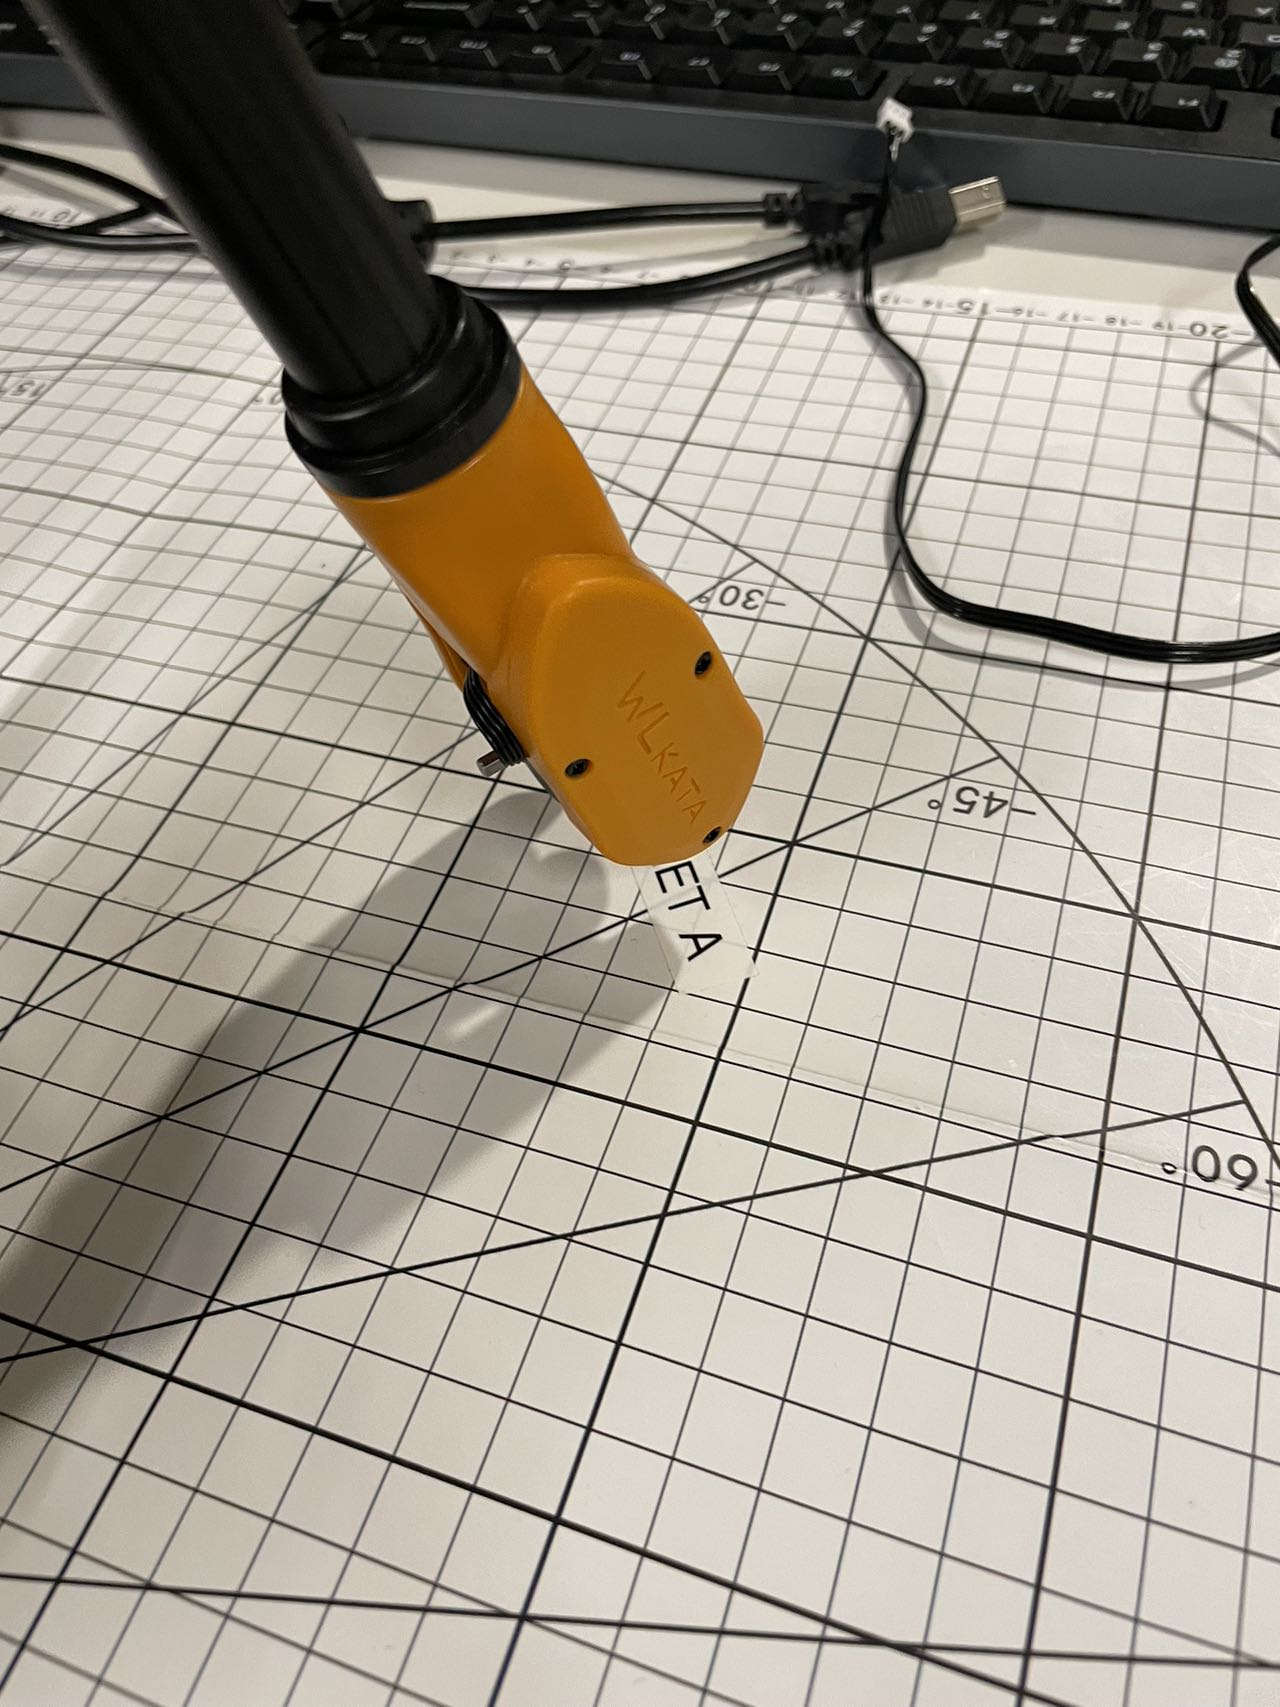
\includegraphics[height=2.5in]{image/2d_linear_a.jpg}
         \caption*{Linear: \texttt{TARGET A}}
     \end{subfigure}
     %
     \hfill
     %
     \begin{subfigure}[b]{0.3\textwidth}
        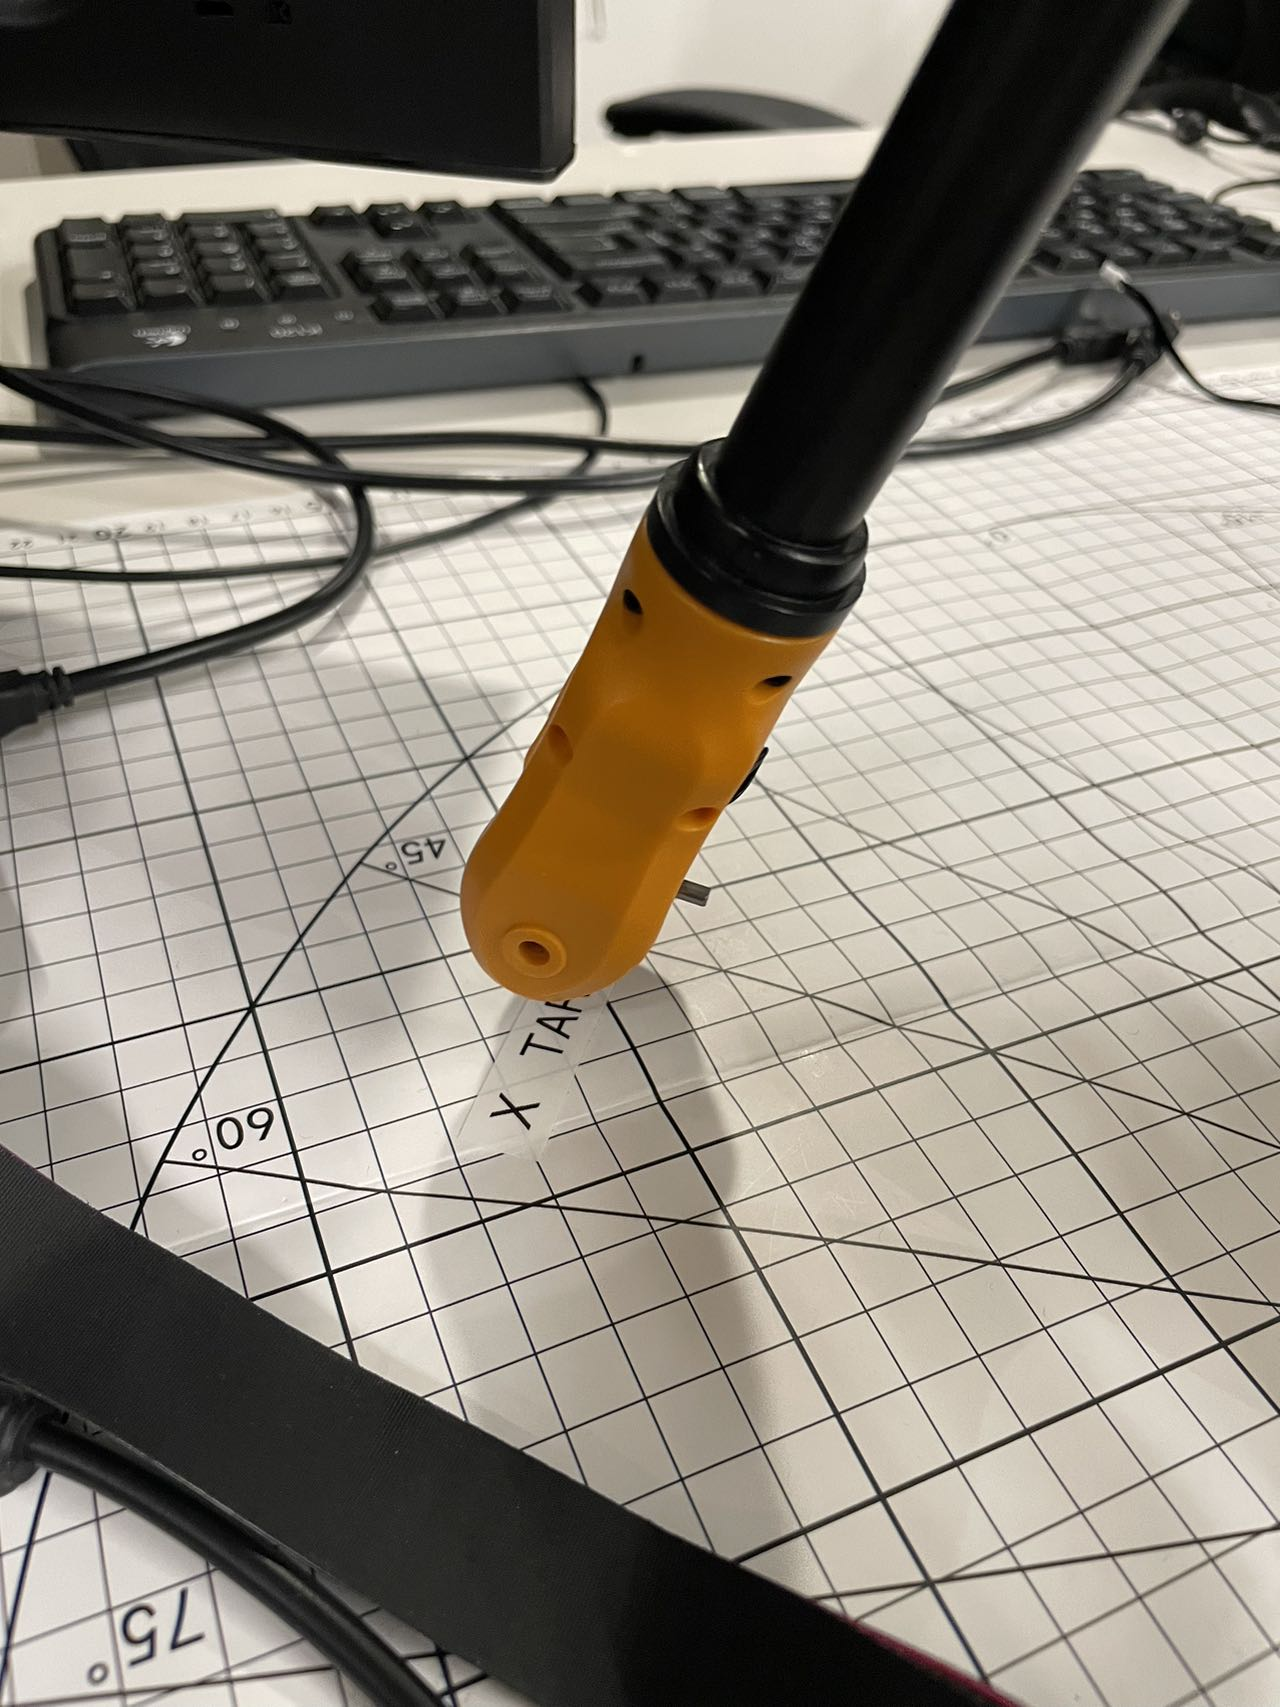
\includegraphics[height=2.5in]{image/2d_linear_b.jpg}
         \caption*{Linear: \texttt{TARGET B}}
     \end{subfigure}
    \caption*{Answer for 2D.}
\end{figure}
%
\begin{minted}{python}
# Again, common header (import/homing etc.) ignored

if sys.argv[1] == 'linear':
    # Go to A
    arm.linear_interpolation(x=130.0,y=150.0,z=10.0)
    time.sleep(2)
    # Interpolate to B
    arm.linear_interpolation(x=-160.0, y=140.0, z=10.0)
\end{minted}

\newpage
\begin{figure}[hb!]
     \centering
    \begin{subfigure}[b]{0.3\textwidth}
        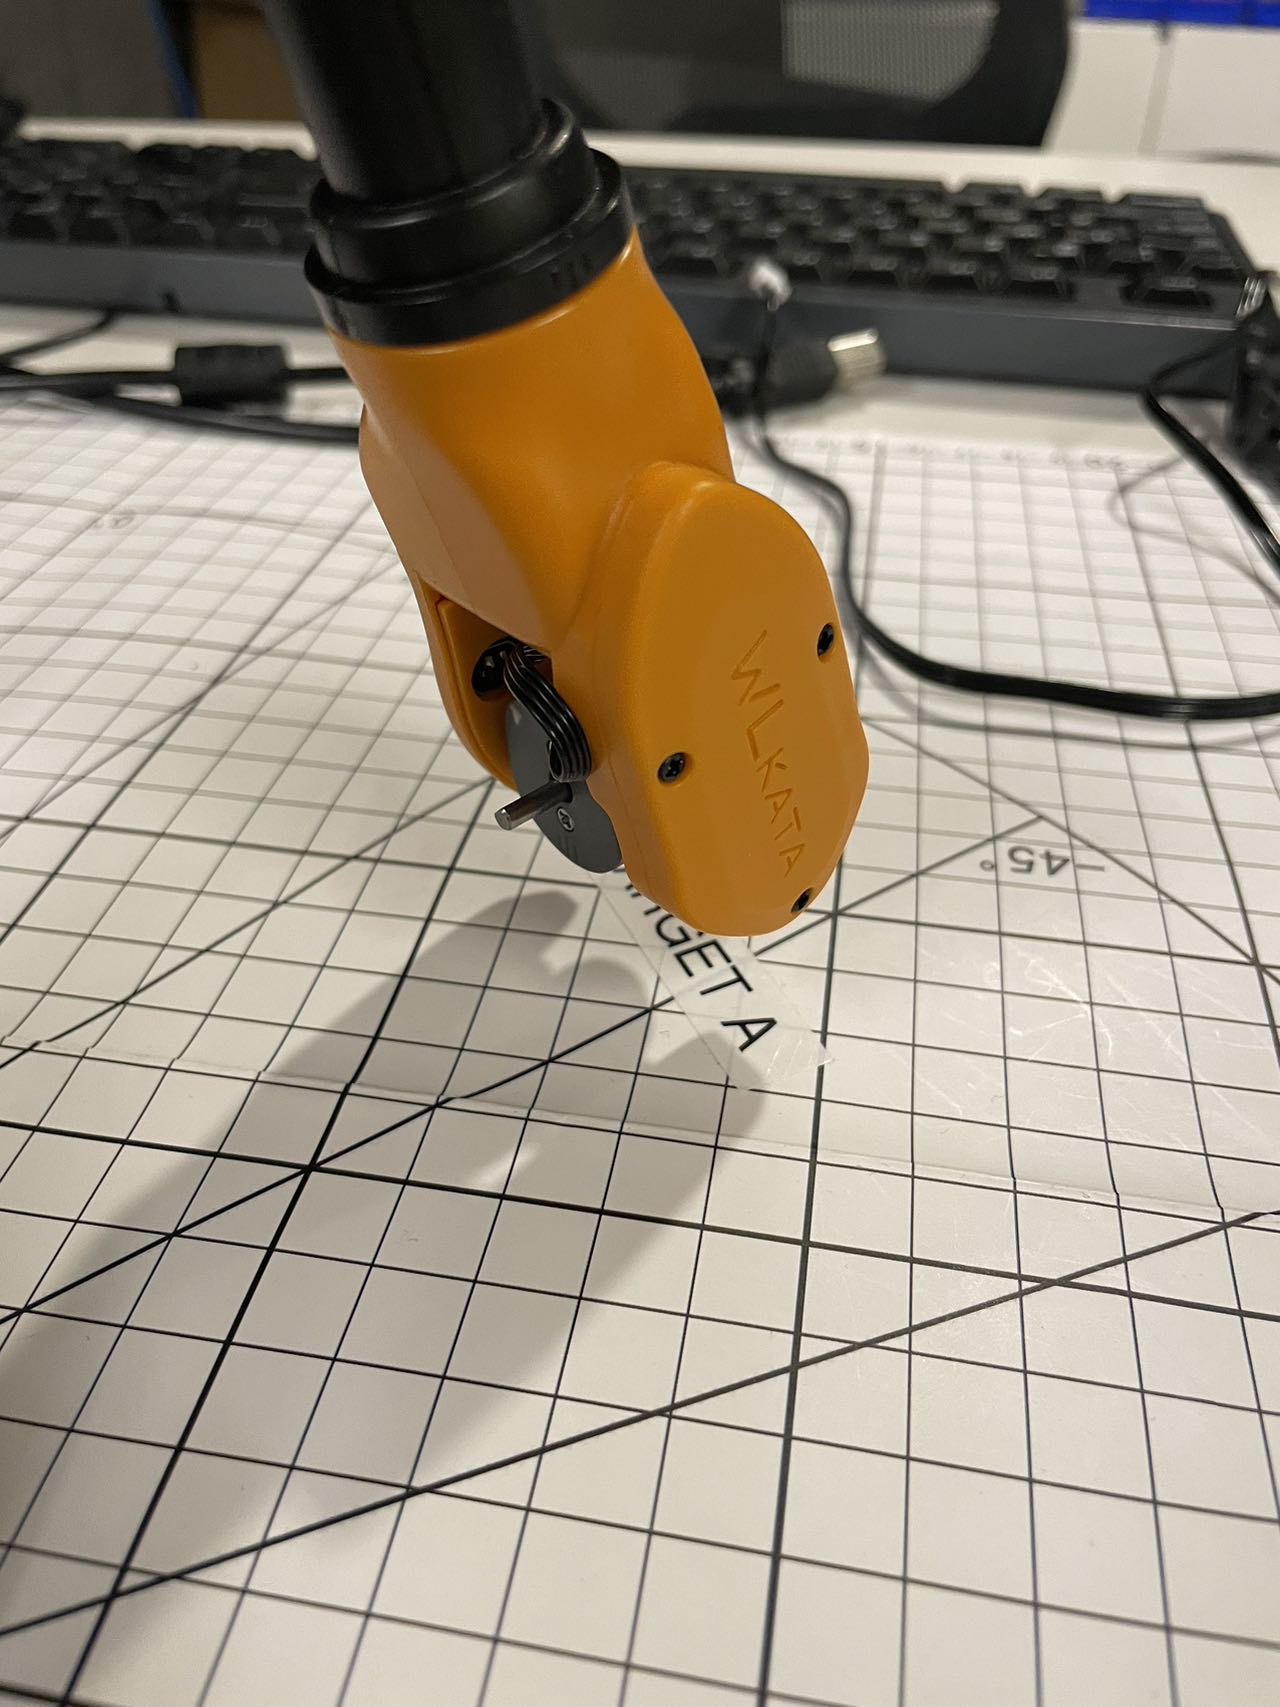
\includegraphics[height=2.5in]{image/2d_door_a.jpg}
         \caption*{Door: \texttt{TARGET A}}
     \end{subfigure}
     %
     \hfill
     %
     \begin{subfigure}[b]{0.3\textwidth}
        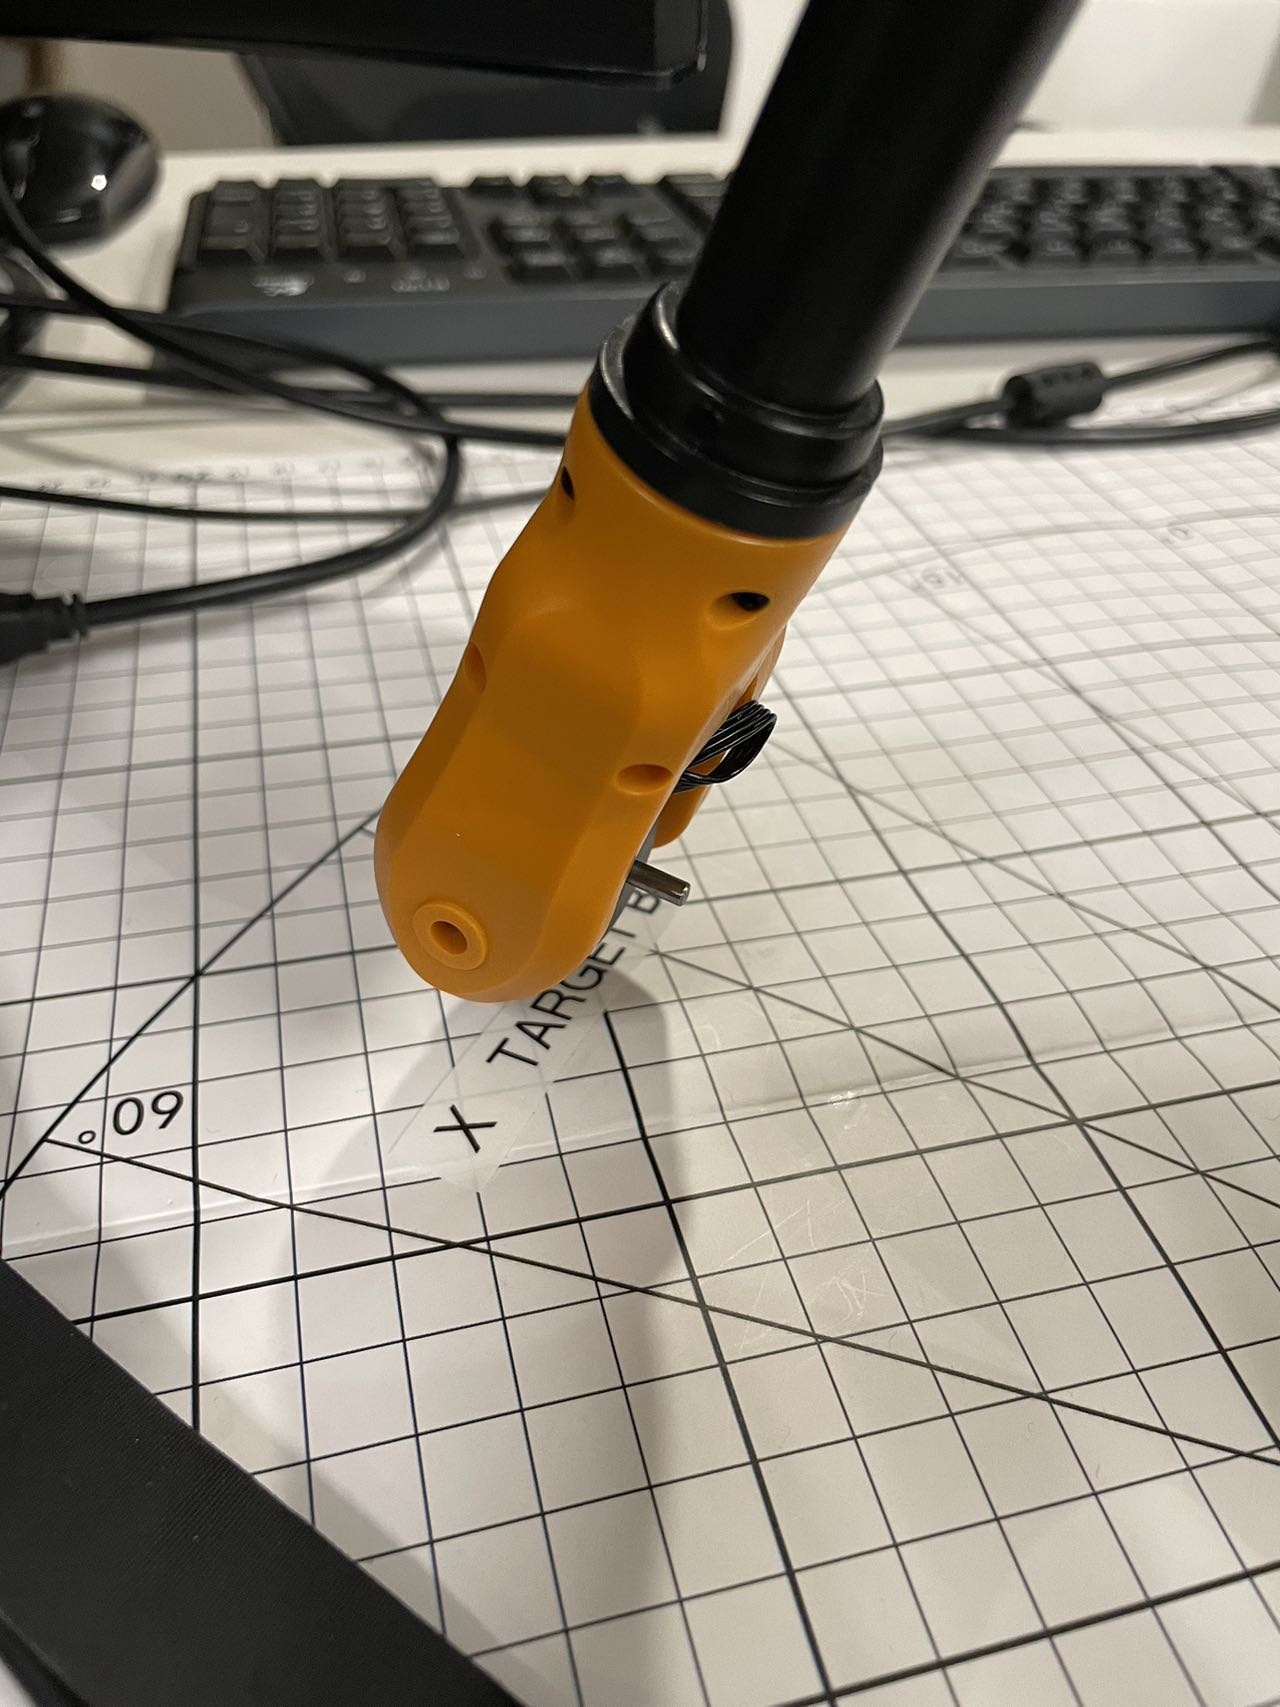
\includegraphics[height=2.5in]{image/2d_door_b.jpg}
         \caption*{Door: \texttt{TARGET B}}
     \end{subfigure}
    \caption*{Answer for 2D.}
\end{figure}
%
\begin{minted}{python}
# Again, common header (import/homing etc.) ignored

if sys.argv[1] == 'door':
    # Set lift distance
    arm.set_door_lift_distance(50)
    # Go to A
    arm.set_tool_pose(x=130.0,y=150.0,z=10.0, wait_ok=True)
    time.sleep(2)
    # Interpolate to B
    arm.door_interpolation(x=-160.0, y=140.0, z=10.0)
\end{minted}

\newpage
\begin{figure}[hb!]
     \centering
    \begin{subfigure}[b]{0.3\textwidth}
        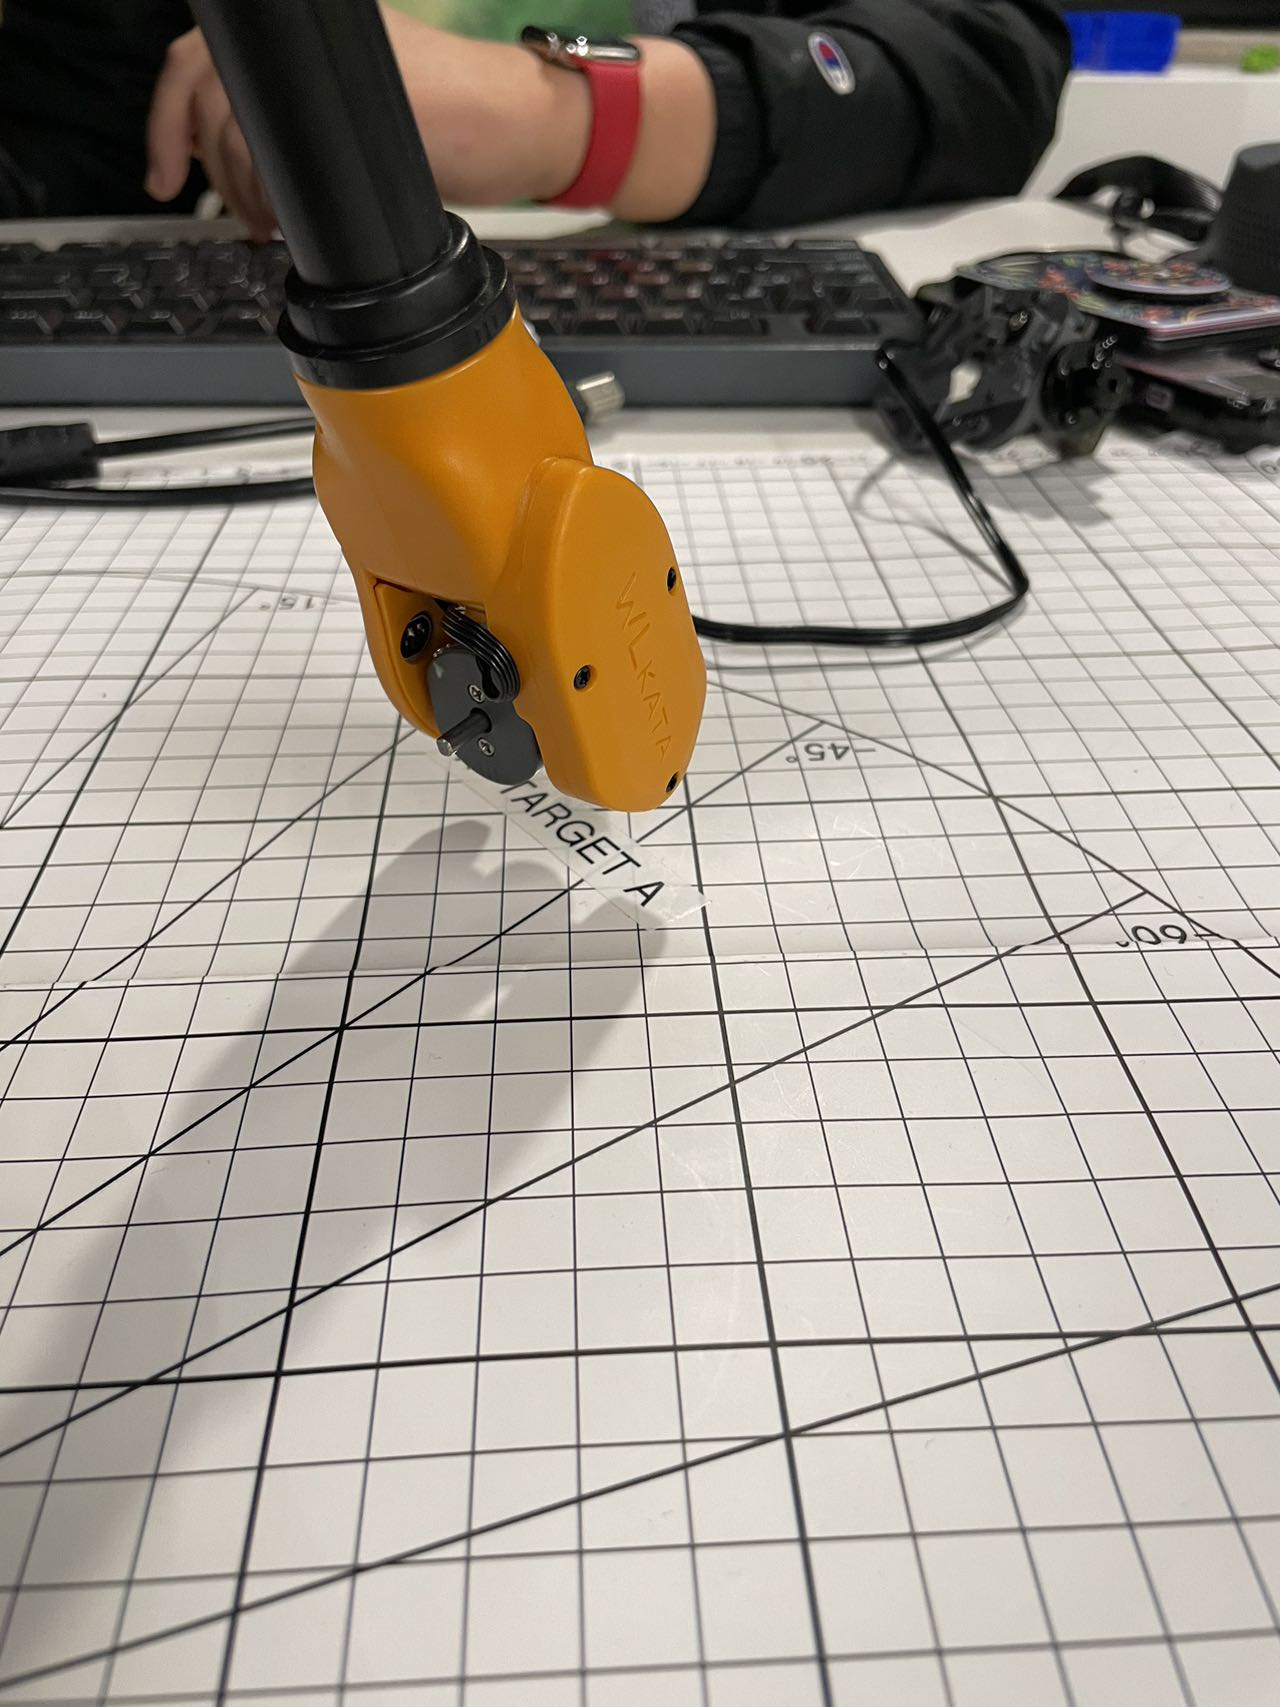
\includegraphics[height=2.5in]{image/2d_circular_a.jpg}
         \caption*{Circular: \texttt{TARGET A}}
     \end{subfigure}
     %
     \hfill
     %
     \begin{subfigure}[b]{0.3\textwidth}
        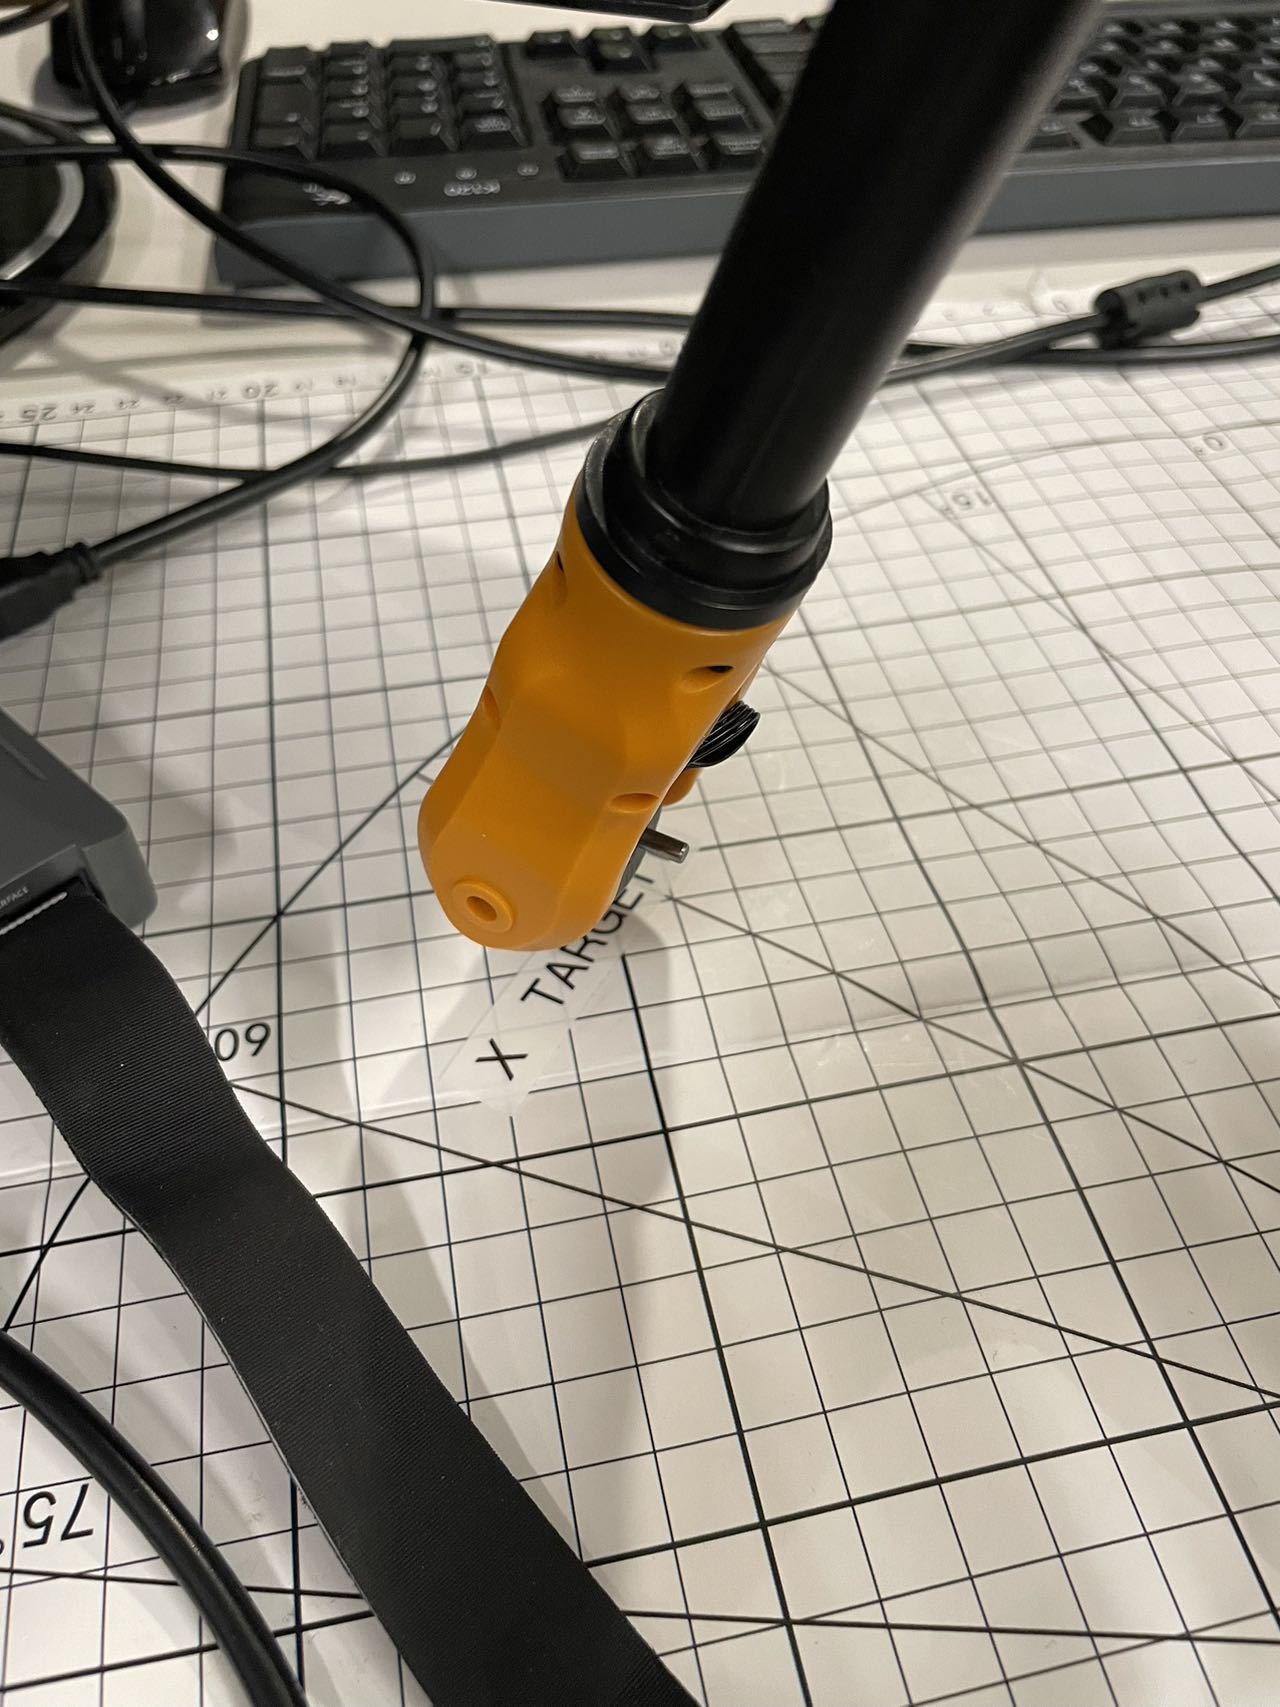
\includegraphics[height=2.5in]{image/2d_circular_b.jpg}
         \caption*{Circular: \texttt{TARGET B}}
     \end{subfigure}
    \caption*{Answer for 2D.}
\end{figure}
%
\begin{minted}{python}
# Again, common header (import/homing etc.) ignored

if sys.argv[1] == 'circular':
    # Go to A
    arm.set_tool_pose(x=130.0,y=150.0,z=10.0, wait_ok=True)
    print(f"Arrived at {arm.pose}")
    time.sleep(2)
    # Interpolate to B
    arm.circular_interpolation(ex=-290, ey=-10, radius=300, \
        is_cw=False, wait_ok=True)
    print(f"Interpolation complete! Now at {arm.pose}")
\end{minted}

\newpage

\paragraph{Additional Space.}
Attached below is the full orginal code used for question 2d.
\begin{minted}{python}
from wlkata_mirobot import WlkataMirobot
import time
import sys

arm = WlkataMirobot(portname='COM3')
arm.home()


if sys.argv[1] == 'p2p':
    # Go to A
    arm.p2p_interpolation(x=130.0,y=150.0,z=10.0, wait_ok=True)
    time.sleep(2)
    # Interpolate to B
    arm.p2p_interpolation(x=-160.0, y=140.0, z=10.0)
if sys.argv[1] == 'linear':
    # Go to A
    arm.linear_interpolation(x=130.0,y=150.0,z=10.0)
    time.sleep(2)
    # Interpolate to B
    arm.linear_interpolation(x=-160.0, y=140.0, z=10.0)
if sys.argv[1] == 'door':
    # Set lift distance
    arm.set_door_lift_distance(50)
    # Go to A
    arm.set_tool_pose(x=130.0,y=150.0,z=10.0)
    time.sleep(2)
    # Interpolate to B
    arm.door_interpolation(x=-160.0, y=140.0, z=10.0)
if sys.argv[1] == 'circular':
    # Go to A
    arm.set_tool_pose(x=130.0,y=150.0,z=10.0, wait_ok=True)
    print(f"Arrived at {arm.pose}")
    time.sleep(2)
    # Interpolate to B
    arm.circular_interpolation(ex=-290, ey=-10, radius=300, is_cw=False, wait_ok=True)
    print(f"Interpolation complete! Now at {arm.pose}")
\end{minted}
Please do not exceed this page for this question.
%%%%%% YOU ANSWER ENDS HERE
